\section{Kết luận đồ án tốt nghiệp}
Trong khuôn khổ đồ án tốt nghiệp, đề tài đã nghiên cứu, thiết kế và xây dựng hệ thống
CityFoodTour - một nền tảng hỗ trợ người dùng khám phá địa điểm ăn uống và xây dựng
hành trình food tour cá nhân hóa.

Hệ thống đã đáp ứng các mục tiêu đề ra thông qua việc triển khai các chức năng chính
bao gồm quản lý người dùng, tìm kiếm và quản lý thông tin quán ăn, xây dựng food tour,
hiển thị thông tin địa điểm trên bản đồ và hỗ trợ gợi ý quán ăn dựa trên sở thích của
người dùng.

Về mặt kỹ thuật, đề tài đã xây dựng hệ thống theo kiến trúc phân tách giữa tầng giao
diện, tầng xử lý nghiệp vụ và tầng dữ liệu, giúp hệ thống có khả năng mở rộng và bảo
trì trong tương lai. Các chức năng được kiểm thử nhằm đánh giá tính đúng đắn, độ ổn
định và khả năng đáp ứng yêu cầu sử dụng.

Bên cạnh các kết quả đạt được, hệ thống vẫn còn một số hạn chế như phạm vi 
dữ liệu quán ăn còn bị giới hạn, khả năng cá nhân hóa của module gợi ý cần 
tiếp tục được cải thiện và một số chức năng nâng cao cần được nghiên cứu thêm.

\section{Hướng phát triển}

Trong tương lai, hệ thống CityFoodTour có thể được tiếp tục mở rộng theo các
hướng sau:

\begin{itemize}

    \item Nghiên cứu khả năng tích hợp thêm các nguồn dữ liệu bên ngoài như
    dịch vụ bản đồ, thông tin địa điểm và dữ liệu đánh giá nhằm nâng cao độ
    chính xác và khả năng cập nhật của hệ thống.
    
    \item Mở rộng và cập nhật cơ sở dữ liệu quán ăn nhằm tăng số lượng địa điểm
    được hỗ trợ, đồng thời cải thiện độ đa dạng của các lựa chọn khi người dùng
    tìm kiếm và xây dựng food tour.

    \item Cải thiện cơ chế gợi ý quán ăn bằng cách bổ sung thêm các tiêu chí
    phù hợp như lịch sử tương tác, đánh giá của người dùng, so sánh các hồ sơ 
    người dùng với nhau mức độ phổ biến của địa điểm và khoảng cách giữa các 
    điểm trong lộ trình.

    \item Hoàn thiện chức năng tối ưu lộ trình food tour bằng cách nghiên cứu
    thêm các phương pháp sắp xếp thứ tự điểm đến phù hợp hơn, giúp giảm thời
    gian di chuyển và nâng cao trải nghiệm của người dùng.

    \item Phát triển ứng dụng trên nền tảng di động nhằm giúp người dùng dễ dàng
    sử dụng hệ thống trong quá trình khám phá và di chuyển giữa các địa điểm
    ăn uống.

    \item Bổ sung thêm các chức năng tương tác cộng đồng như theo dõi người
    dùng khác, hệ thống gửi tin nhắn nhằm thuận tiện cho việc chia sẻ và gợi ý
    cho bạn bè

\end{itemize}
% \begin{figure}[H]
%     \centering
%     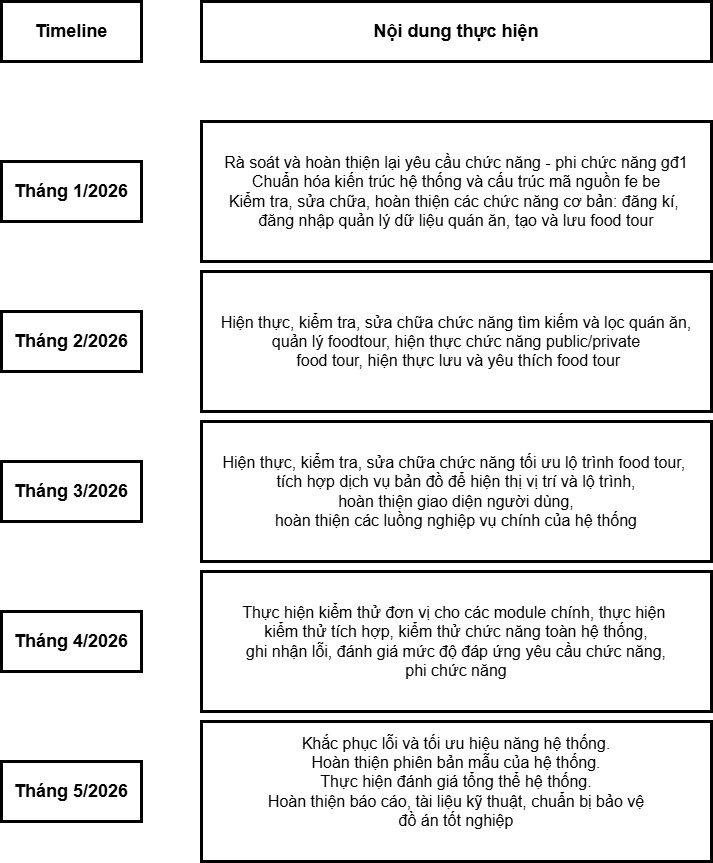
\includegraphics[width=0.85\linewidth]{img/timeline.png}
%     \caption{Timeline Đồ án tốt nghiệp}
% \end{figure}

% Trong giai đoạn đồ án tốt nghiệp, công việc được phân công cụ thể giữa các sinh viên
% tham gia thực hiện nhằm đảm bảo tiến độ và hiệu quả triển khai hệ thống. 

% \begin{itemize}[label=\textbullet]
%     \item Trần Minh Quang phụ trách phát triển tầng giao diện người dùng (frontend). 
%     \item Đặng Thanh Vũ chịu trách nhiệm chính trong việc phát triển tầng backend và thiết kế, hiện thực cơ sở dữ liệu. 
%     \item Nguyễn Duy Ngọc tham gia hỗ trợ và thực hiện đồng thời ở cả frontend, backend và cơ sở dữ liệu,
% đóng vai trò phối hợp và tích hợp các thành phần của hệ thống.
% \end{itemize}


